\documentclass[12pt,a4paper,landscape]{article}

% -- Package Imports --
\usepackage[utf8]{inputenc}
\usepackage[T1]{fontenc}
\usepackage{booktabs}
\usepackage{graphicx}
\graphicspath{{./}{./images/}{../sections/images/}}
\usepackage{longtable}
\usepackage{newtxtext} % Times-like text font
\usepackage{newtxmath} % Times-like math
\usepackage{setspace}
\usepackage{array}
\usepackage{multirow}
\usepackage{tabularx}
\usepackage{xcolor}
\usepackage{colortbl}
\usepackage{geometry}
\usepackage[colorlinks=true,linkcolor=blue,citecolor=blue,urlcolor=blue]{hyperref}
\usepackage{float}
\usepackage{enumitem}
\usepackage{fancyhdr}
\usepackage{pdflscape}
\usepackage{makecell}
\usepackage{caption}

% -- Document Setup --
\geometry{a4paper, margin=2.5cm}
\setstretch{1.5}
\setlength{\parindent}{0pt}
\setlength{\parskip}{6pt}

% -- Table Column Types --
\newcolumntype{L}[1]{>{\raggedright\arraybackslash}p{#1}}
\newcolumntype{C}[1]{>{\centering\arraybackslash}p{#1}}
\newcolumntype{R}[1]{>{\raggedleft\arraybackslash}p{#1}}

% -- Header and Footer --
\pagestyle{fancy}
\fancyhf{}
\fancyhead[L]{PhD Protocol Appendices}
\fancyhead[R]{Craig Parker}
\fancyfoot[C]{Page \thepage}
\renewcommand{\headrulewidth}{0.4pt}
\renewcommand{\footrulewidth}{0.4pt}

\begin{document}

\begin{center}
    \Large\textbf{APPENDICES}\\[0.5em]
    \large\textbf{Urban Heat, Health, and Vulnerability in South African Cities:}\\
    \large\textbf{A Mixed-Methods Approach to Predictive Modeling}\\[0.5em]
    \normalsize Craig Parker\\
    \normalsize University of Cape Town\\
    \normalsize April 2025
\end{center}

\section*{Appendix A: Supplementary Figures}

\subsection*{A.1 Temperature Trends in Johannesburg}
\begin{figure}[H]
    \centering
    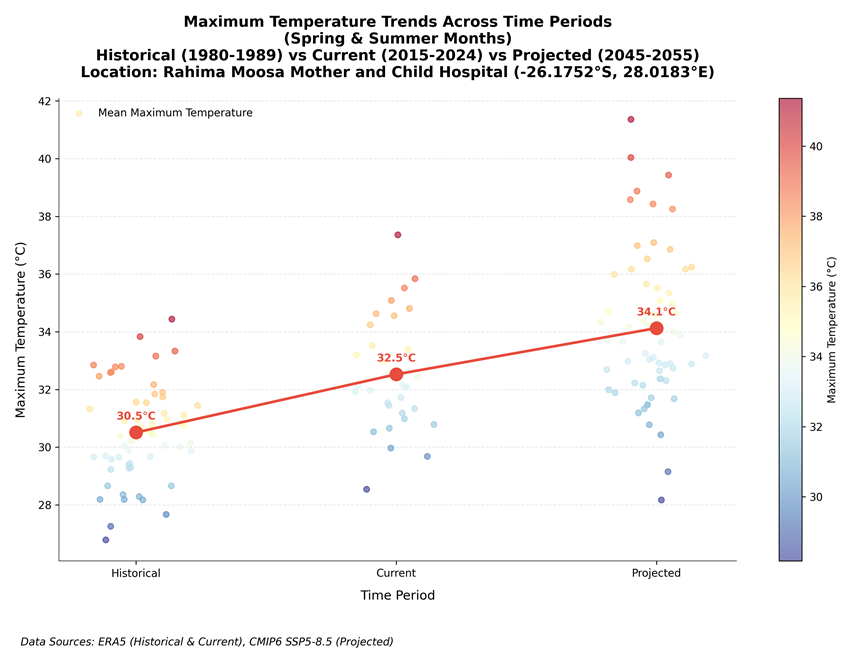
\includegraphics[width=0.8\textwidth]{images/Max_temp_trends_across_time_periods.png}
    \caption{Maximum temperature trends across different time periods in Johannesburg, showing increasing frequency and intensity of extreme heat events.}
    \label{fig:temp_trends}
\end{figure}

\subsection*{F.9 Project Timeline (GANTT Chart)}
\begin{figure}[H]
    \centering
    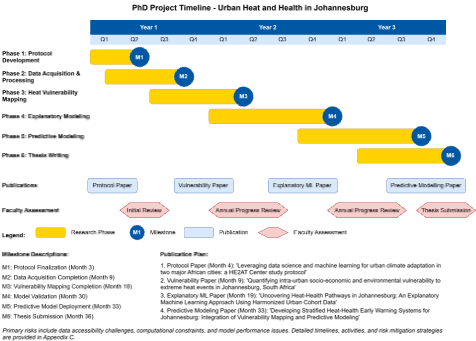
\includegraphics[width=0.9\textwidth]{images/GNT.png}
    \caption{Detailed project timeline showing research phases, milestones, and deliverables across the PhD duration.}
    \label{fig:gantt}
\end{figure}

\begin{center}
    \Large\textbf{APPENDIX DOCUMENT}\\[0.5em]
    \normalsize\textit{The following tables and appendices are separated from the main document to support word count requirements.}
\end{center}

\section*{Data Management and Methodological Tables for HE\textsuperscript{2}AT Center Research}

\subsection*{Table 1: Data Sources and Applications}
\begin{longtable}{p{3cm}p{3cm}p{4cm}p{3cm}}
\toprule
\textbf{Source} & \textbf{Type} & \textbf{Variables} & \textbf{Application} \\
\midrule
\endhead

Weather Service & Historical & Temperature, humidity & Climate analysis \\
\midrule
Satellite & Remote sensing & Land surface temperature & Heat mapping \\
\bottomrule
\caption{Primary data sources for the heat vulnerability analysis}
\end{longtable}

\end{document}
